% !TEX root = ../tfg_etsiinf_NombreApellidos.tex
\chapter{Aplicación y validación de la arquitectura} \label{chp:pruebas}

Este capítulo aplica la infraestructura desarrollada a una tarea concreta de
control de velocidad para un UAV simulado. Mientras que el
Capítulo~\ref{chp:implementacion} verifica que los componentes están correctamente
implementados y pueden producir transiciones físicas válidas, aquí se analiza si
la arquitectura permite entrenar una política PPO para alcanzar un objetivo
relativo mediante comandos continuos de velocidad y guiñada. Esta aplicación
convierte la arquitectura en una infraestructura de experimentación: las observaciones, las
acciones, la recompensa, el reinicio y la monitorización se ejercitan de forma
conjunta bajo una misma tarea de control.

La validación distingue la disponibilidad de la infraestructura del
comportamiento de la política. Un entrenamiento solo es interpretable si cada
episodio comienza en un estado verificable y las acciones modifican físicamente
el estado del vehículo; sobre esa condición se pueden evaluar la aproximación al
objetivo, las terminaciones y las métricas de aprendizaje. Las secciones
siguientes presentan la formulación de la tarea, las salvaguardas y la
configuración empleada, así como los criterios con los que se analizan las
ejecuciones.

\section{Propósito y alcance de la aplicación} \label{sct:aplicacion:alcance}

La aplicación de validación consiste en entrenar una política PPO que recibe el
estado relativo del UAV respecto de un objetivo y emite velocidades lineales y
de guiñada. El entrenamiento se ejecuta sobre \texttt{AS2TestEnv}, que traduce
cada acción de la política en una referencia para Aerostack2 y devuelve la
observación, la recompensa y el estado de terminación correspondientes. De este
modo, la tarea exige simultáneamente que el canal de control sea accionable, que
el ciclo de reinicio sea fiable y que la formulación de aprendizaje proporcione
una señal útil para la navegación local.

Esta aplicación no se plantea como una demostración aislada de que el proceso de
entrenamiento se inicia, sino como una validación integrada del objetivo del
trabajo. Una ejecución adecuada debe generar episodios trazables, conservar las
condiciones de seguridad y permitir evaluar si la política reduce la distancia
al objetivo y alcanza la región de éxito. Los apartados posteriores concretan
esta tarea mediante la formulación de control, la recompensa, el curriculum, las
protecciones de frontera, la configuración de PPO y las métricas de aceptación.

\section{Formulación de la tarea de control} \label{sct:aplicacion:formulacion}

El problema de control se formula como una tarea de navegación local hacia un
objetivo relativo. En este contexto, navegación local significa que el agente no
recibe una misión global completa ni una trayectoria predefinida con todos sus
puntos intermedios, sino la relación geométrica entre el estado actual del UAV y
un objetivo inmediato. A partir de esa relación, el agente debe emitir comandos
de velocidad que acerquen el vehículo al objetivo y mantengan una orientación
coherente con la dirección de desplazamiento.

Antes de definir formalmente las observaciones y acciones, conviene distinguir
las magnitudes básicas que describen el movimiento de un multirrotor. La posición
indica dónde se encuentra el UAV en el espacio; la velocidad indica cómo cambia
esa posición; y la orientación describe la rotación del vehículo respecto a sus
ejes. En un dron se suelen emplear tres ángulos principales, denominados
\emph{roll}, \emph{pitch} y \emph{yaw}. El \emph{roll} representa la inclinación lateral,
el \emph{pitch} la inclinación hacia delante o hacia atrás, y el \emph{yaw} la
rotación alrededor del eje vertical. La Figura~\ref{fig:diseno:pose_drone}
resume esta idea de pose del dron mediante una representación conceptual tomada
de ResearchGate.\footnote{Imagen disponible en ResearchGate:
\url{https://www.researchgate.net/figure/A-conceptual-representation-of-drone-pose-A-drone-here-represented-by-a-DJI-Mavic-2-is_fig1_356985671}. Según la página consultada, la figura aparece con licencia Creative Commons Attribution-NonCommercial-ShareAlike 4.0 International.}

\begin{figure}[t]
    \centering
    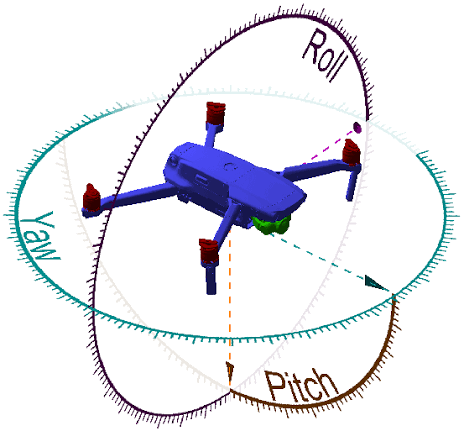
\includegraphics[width=0.58\textwidth]{images/drone_pose_roll_pitch_yaw.png}
    \caption{Representación conceptual de la pose de un dron mediante los ángulos
    de \emph{roll}, \emph{pitch} y \emph{yaw}. Fuente: ResearchGate.}
    \label{fig:diseno:pose_drone}
\end{figure}

En el presente trabajo no se controla directamente la actitud completa del dron
ni las velocidades de giro de cada rotor. La acción se define a un nivel de abstracción superior, en el que el agente
genera velocidades lineales y una velocidad de guiñada. Esta elección sitúa el
aprendizaje por refuerzo por encima del control de bajo nivel y delega en
Aerostack2 la ejecución de los comandos sobre el simulador. Desde el punto de
vista del diseño, esta separación reduce la
complejidad del problema aprendido y mantiene la compatibilidad con la interfaz
de control de velocidad disponible.

La formulación distingue también entre la dirección frontal del UAV y la
dirección real de avance. Un dron puede desplazarse hacia un objetivo aunque su
eje frontal no esté alineado con la trayectoria seguida. El criterio de
\emph{path-facing}, ilustra la
diferencia entre ambas magnitudes y la relación con el error de guiñada. En la
formulación final de la solución no se exige el seguimiento de una trayectoria: la guiñada se
considera únicamente al evaluar el éxito terminal. La
Figura~\ref{fig:aplicacion:target_path_facing} representa esta relación
geométrica.


\begin{figure}[t]
\centering
\shorthandoff{<>}
\begin{tikzpicture}[
    x=1cm,
    y=1cm,
    axis/.style={-{Latex[length=2mm]}, thick, gray},
    rel/.style={-{Latex[length=2.5mm]}, very thick, blue},
    front/.style={-{Latex[length=2.5mm]}, very thick, green!55!black},
    path/.style={-{Latex[length=2.5mm]}, very thick, orange!85!black},
    helper/.style={dashed, gray!65},
    label/.style={font=\small},
    smalllabel/.style={font=\scriptsize}
]

\coordinate (uav) at (0,0);
\coordinate (target) at (6.2,2.5);
\coordinate (front) at (2.0,0.35);
\coordinate (pathvec) at (2.0,0.85);

% Axes
\draw[axis] (-0.6,0) -- (7.0,0) node[right, label] {$x$};
\draw[axis] (0,-0.5) -- (0,3.2) node[above, label] {$y$};

% UAV and target
\begin{scope}[shift={(uav)}, rotate=10]
    \draw[fill=gray!20, thick] (0.48,0) -- (-0.32,0.22) -- (-0.32,-0.22) -- cycle;
\end{scope}
\node[label, below left=0.12cm of uav] {UAV};
\filldraw[red] (target) circle (2.3pt);
\node[label, red, above right=0.05cm of target] {objetivo};

% Projection helpers
\draw[helper] (target) -- (6.2,0);
\draw[helper] (target) -- (0,2.5);

% Main vectors
\draw[rel] (uav) -- (target);
\draw[front] (uav) -- (front);
\draw[path] (uav) -- (pathvec);

% Angle arcs
\draw[->, thick, green!55!black] (0.85,0) arc[start angle=0,end angle=10,radius=0.85];
\draw[->, thick, orange!85!black] (1.2,0) arc[start angle=0,end angle=23,radius=1.2];
\draw[<->, thick, red!70!black] (1.55,0.27) arc[start angle=10,end angle=23,radius=1.58];

% Compact legend below the plot, outside the geometry
\begin{scope}[shift={(0,-1.25)}]
    \draw[rel] (0.0,0.0) -- (0.65,0.0);
    \node[label, anchor=west] at (0.85,0.0) {vector relativo $(d_x,d_y)$};

    \draw[front] (5.2,0.0) -- (5.85,0.0);
    \node[label, anchor=west] at (6.05,0.0) {dirección frontal};

    \draw[path] (0.0,-0.55) -- (0.65,-0.55);
    \node[label, anchor=west] at (0.85,-0.55) {dirección de avance};

    \draw[<->, thick, red!70!black] (5.2,-0.55) -- (5.85,-0.55);
    \node[label, anchor=west] at (6.05,-0.55) {error $e_{\mathrm{yaw}}$};
\end{scope}

\end{tikzpicture}
\shorthandon{<>}
\caption{Relación geométrica entre el UAV, el objetivo relativo, la dirección de
avance y la orientación de guiñada utilizada en el criterio de
\emph{path-facing}.}
\label{fig:aplicacion:target_path_facing}
\end{figure}

La acción se define mediante el vector continuo
\[
    a = [v_x, v_y, v_z, v_{\mathrm{yaw}}].
\]
Las tres primeras componentes representan velocidades lineales en los ejes
cartesianos y la cuarta representa la velocidad angular de guiñada. El espacio de
acciones se acota mediante los parámetros \texttt{max\_vel} y
\texttt{max\_yaw\_vel}, lo que introduce una restricción explícita de diseño
sobre la magnitud de las órdenes que el agente puede emitir. Esta acotación es
necesaria porque una política de aprendizaje por refuerzo puede proponer acciones
arbitrarias dentro de su espacio de salida, mientras que el sistema físico o
simulado solo debe recibir comandos dentro de un rango admisible.

La observación se define mediante el vector relativo
\[
    o = [d_x, d_y, d_z, d_{\mathrm{yaw}}].
\]
Cada componente se normaliza en el intervalo $[-1, 1]$. Las tres primeras
componentes codifican el desplazamiento relativo hacia el objetivo, y la cuarta
codifica la diferencia relativa de guiñada. La normalización reduce la dependencia
respecto a la escala concreta del escenario y proporciona al agente entradas con
rangos homogéneos, una condición práctica para estabilizar el tratamiento de las
observaciones por parte del algoritmo de aprendizaje.

\section{Recompensa y condiciones de finalización} \label{sct:aplicacion:recompensa}

La recompensa final usada en la fase de experimentación principal se diseña para
mantener una señal mínima e interpretable. En
cada paso se penaliza únicamente la distancia normalizada al objetivo. Para ello, si
$d_t$ representa la distancia euclídea entre el UAV y el objetivo, y
$d_{\max}$ representa la distancia máxima de normalización. A partir de ambas
magnitudes se obtiene
\begin{equation}
    d_{\mathrm{norm}} = \min\left(\frac{d_t}{d_{\max}}, 1\right),
    \qquad
    r_{\mathrm{dist}} = -d_{\mathrm{norm}}.
\end{equation}
En la interfaz Gymnasium implementada, $d_{\max}$ se calcula a partir del límite espacial de
posición del escenario, de forma que la distancia normalizada queda acotada en el
intervalo $[0,1]$.

La interfaz Gymnasium conserva la capacidad de calcular términos adicionales, como progreso,
seguridad vertical o coherencia de guiñada con la dirección de movimiento. Sin
embargo, esos términos se desactivan a partir de Exp010 y en toda la campaña
principal para evitar que el agente optimice una recompensa de shaping distinta
de la tarea principal. La guiñada se mantiene como requisito terminal suave. Cuando el UAV alcanza la
región objetivo, la bonificación de éxito se reduce en función del error de
guiñada. Si
$e_{\mathrm{yaw}}$ representa el error angular normalizado, la recompensa terminal
de éxito se calcula mediante
\begin{equation}
    r_{\mathrm{success}} =
    R_{\mathrm{success}} -
    w_{\mathrm{yaw}} \frac{|e_{\mathrm{yaw}}|}{\pi}.
\end{equation}

La expresión final aplicada desde Exp010 en adelante incorpora las
condiciones terminales del episodio de la forma siguiente.
\begin{equation}
    r_t =
    \begin{cases}
        -P_{\mathrm{oob}}, & \text{si el UAV sale de los límites del escenario},\\
        -P_{\mathrm{oob}}, & \text{si el UAV entra en baja altitud insegura},\\
        r_{\mathrm{success}}, &
            \text{si } d_t < d_{\mathrm{threshold}},\\
        -d_{\mathrm{norm}}, & \text{en el resto de pasos}.
    \end{cases}
\end{equation}
El truncamiento por alcanzar \texttt{max\_steps} no introduce una recompensa
adicional, sino que limita la duración del episodio cuando no se ha alcanzado una
condición terminal. El Cuadro~\ref{tab:aplicacion:componentes_recompensa} resume los
componentes de esta formulación y su efecto esperado.

\begin{table}[t]
\centering
\small
\setlength{\tabcolsep}{4pt}
\renewcommand{\arraystretch}{1.15}
\begin{tabular}{p{0.24\textwidth} p{0.25\textwidth} p{0.19\textwidth} p{0.22\textwidth}}
\hline
\textbf{Componente} & \textbf{Expresión} & \textbf{Condición} & \textbf{Efecto esperado} \\
\hline

Penalización por distancia &
$r_{\mathrm{dist}} = -d_{\mathrm{norm}}$ &
En cada paso &
Favorece que el UAV reduzca progresivamente la distancia al objetivo. \\

Bonificación por éxito &
$R_{\mathrm{success}} - w_{\mathrm{yaw}} |e_{\mathrm{yaw}}|/\pi$ &
Si $d_t < d_{\mathrm{threshold}}$ &
Premia alcanzar la región objetivo y reduce la bonificación si la guiñada terminal es inadecuada. \\

Penalización por salida de límites &
$-P_{\mathrm{oob}}$ &
Si el UAV supera los límites del escenario &
Desincentiva trayectorias inseguras o alejadas de la zona de entrenamiento. \\

Penalización por baja altitud insegura &
$-P_{\mathrm{oob}}$ &
Si el UAV desciende por debajo del umbral inseguro &
Evita que el aprendizaje explote estados cercanos al suelo o físicamente no válidos. \\

Truncado temporal &
Sin recompensa adicional &
Si se alcanza el número máximo de pasos &
Limita la duración del episodio cuando no se alcanza una condición terminal. \\

\hline
\end{tabular}
\caption{Componentes de la función de recompensa y condiciones de finalización de la interfaz Gymnasium.}
\label{tab:aplicacion:componentes_recompensa}
\end{table}

\section{Curriculum de distancia} \label{sct:aplicacion:curriculum}

Con la recompensa mínima $-d_{\mathrm{norm}}$, la única señal positiva del
problema es la bonificación terminal, y su densidad depende de la probabilidad de
que la exploración alcance la esfera de éxito de 0,4 m. Con separaciones
inicio--objetivo de hasta 5 m esa probabilidad es demasiado baja para arrancar el
gradiente con la tasa de aprendizaje configurada. El diseño adopta por ello un
curriculum de distancia \cite{bengio2009curriculum} en tres etapas: la primera acota la separación máxima a
2,5 m, de modo que un vuelo directo requiere del orden de 25 pasos; las dos
siguientes amplían el límite a 3,5 m y finalmente a 5,0 m. Cada
etapa se inicializa con el modelo final de la anterior (\emph{warm start}) y
todas mantienen la separación mínima de 1,0 m, de forma que la distribución de
episodios de una etapa contiene a la anterior y la política no olvida los
objetivos cercanos al aprender los lejanos.

\section{Protecciones de frontera} \label{sct:aplicacion:guards}

La observación relativa tiene una consecuencia de diseño que los primeros
experimentos hicieron explícita y es que el agente no puede percibir los límites del
escenario. Una terminación por salida de límites es, desde el punto de vista de
la política, un castigo imprevisible aplicado en estados que no se distinguen de
los estados seguros, por lo que la función de valor no puede anticiparla. Además,
cada una de estas terminaciones obliga a un reinicio mediante el servicio del
simulador, con un coste de decenas de segundos y efectos acumulativos sobre la
plataforma. Por ambos motivos, el diseño sustituye la muerte en frontera por una
protección activa: un \emph{guard} de acción que, cerca de los límites, reemplaza
la componente de velocidad saliente por un empuje hacia el interior.

El guard se diseña con disparo predictivo. La versión reactiva, que actúa cuando
la posición cruza una línea de guardia, resultó insuficiente en el eje vertical ya que
la plataforma invierte la velocidad con lentitud y la inercia atraviesa el margen
antes de que la orden correctora surta efecto. Por ello el disparo evalúa la
posición \emph{predicha}, calculada como posición actual más velocidad medida por
un horizonte de anticipación, y el empuje vertical utiliza la autoridad completa
de velocidad disponible. Las terminaciones por salida de límites y por baja
altitud se conservan intactas como red de seguridad final, pero con el guard
activo pasan de ser el desenlace dominante (80--93\,\% de los episodios en
Exp010--Exp011) a ser residuales, lo que elimina a la vez el ruido inaprendible
de la recompensa y la mayor parte de los reinicios costosos.

\section{Extensión a ejecución vectorizada} \label{sct:aplicacion:vectorizacion}

La ejecución vectorizada se diseña para permitir varias instancias lógicas del
entorno sobre un único simulador compartido. El diseño utiliza espacios de nombres
diferenciados, \texttt{drone0} a \texttt{droneN}, de forma que cada UAV simulado
pueda ser identificado y gobernado de manera independiente dentro de la misma
infraestructura ROS 2. Esta organización reduce la necesidad de duplicar toda la
infraestructura del simulador, pero exige tratar con cuidado la inicialización de
ROS 2, los nombres de los drones y la sincronización entre episodios.

La Figura~\ref{fig:aplicacion:vectorizacion} resume esta organización. Cada
instancia lógica mantiene su propio espacio de nombres, pero todas comparten la
infraestructura física de simulación, por lo que sus reinicios y sus tiempos de
paso deben coordinarse.

\begin{figure}[t]
\centering
\shorthandoff{<>}
\begin{tikzpicture}[
    node distance=1.1cm and 1.4cm,
    block/.style={
        rectangle,
        rounded corners,
        draw,
        align=center,
        minimum width=2.8cm,
        minimum height=0.8cm,
        font=\small
    },
    smallblock/.style={
        rectangle,
        rounded corners,
        draw,
        align=center,
        minimum width=2.4cm,
        minimum height=0.7cm,
        font=\small
    },
    arrow/.style={-{Latex[length=2mm]}, thick}
]

\node[block] (vec) {Entorno vectorizado\\\texttt{SyncVectorEnv}/\texttt{DummyVecEnv}};

\node[smallblock, below left=of vec] (env0) {Instancia 0\\\texttt{drone0}};
\node[smallblock, below=of vec] (env1) {Instancia 1\\\texttt{drone1}};
\node[smallblock, below right=of vec] (env2) {Instancia 2\\\texttt{drone2}};

\node[block, below=2.0cm of env1] (ros) {ROS 2\\espacios de nombres};
\node[block, below=of ros] (sim) {AS2 Multirotor\\Simulator compartido};

\draw[arrow] (vec) -- (env0);
\draw[arrow] (vec) -- (env1);
\draw[arrow] (vec) -- (env2);

\draw[arrow] (env0) -- (ros);
\draw[arrow] (env1) -- (ros);
\draw[arrow] (env2) -- (ros);

\draw[arrow] (ros) -- (sim);

\node[draw, dashed, rounded corners, fit=(env0)(env1)(env2), inner sep=0.25cm,
      label={[font=\small]right:Instancias lógicas del entorno}] {};

\end{tikzpicture}
\shorthandon{<>}
\caption{Extensión vectorizada mediante instancias lógicas asociadas a espacios
de nombres diferenciados sobre una infraestructura de simulación compartida.}
\label{fig:aplicacion:vectorizacion}
\end{figure}

La elección del mecanismo de vectorización viene determinada por una propiedad
del simulador: opera en tiempo de reloj real, de modo que cada paso del entorno
consume la duración física configurada (0,2 s) con independencia del proceso que
lo invoque. Esta propiedad invalida en este sistema el razonamiento habitual a
favor de la vectorización secuencial (\texttt{SyncVectorEnv} en Gymnasium,
\texttt{DummyVecEnv} en Stable-Baselines3), cuyo beneficio procede de agrupar las
observaciones para una única inferencia por lotes: con un simulador de reloj
real, $N$ entornos secuenciales tardan $N$ veces el paso físico en producir $N$
muestras, es decir, el mismo caudal de muestreo que un solo entorno. Por ello el
diseño adopta \texttt{SubprocVecEnv}, que ejecuta los pasos de los $N$ entornos
en paralelo real manteniendo la inferencia por lotes, con la expectativa
(verificada experimentalmente) de multiplicar el muestreo por el número de
drones.

El paso vectorizado en paralelo introduce, sin embargo, un modo de fallo propio
de los simuladores de reloj real, el avance en \emph{lockstep}. Cuando uno de los
entornos ejecuta su reinicio, es una operación que tarda decenas de
segundos, el paso vectorizado queda bloqueado para todos; durante ese intervalo
los demás drones no reciben órdenes nuevas mientras el mundo sigue avanzando, y
el controlador de Aerostack2 mantiene la última referencia de velocidad como
consigna activa. El diseño incorpora por ello un mecanismo de vigilancia
(\emph{watchdog}) de comandos inactivos, es decir,si un entorno en vuelo supera un umbral
de tiempo sin emitir referencias de movimiento, el mecanismo publica una consigna
de velocidad nula de forma periódica hasta que el flujo normal de comandos se
reanuda. El umbral se dimensiona por encima de la duración del paso, de modo que
el mecanismo permanece inerte durante la operación normal y solo actúa en los
huecos de \emph{lockstep}; en ejecución monodron queda desactivado y el
comportamiento del entorno es idéntico al de la fase anterior.

\section{Configuración del entrenamiento PPO} \label{sct:aplicacion:ppo}

La configuración de PPO se materializa en
\texttt{configs/train\_ppo.yaml}. El Capítulo~\ref{chp:state-of-the-art}
justifica la elección del algoritmo; esta sección se limita a documentar cómo se
parametriza su uso dentro de la arquitectura implementada y cómo se preserva la
trazabilidad de cada ejecución.

La configuración se divide en tres bloques principales. El bloque
\texttt{experiment} define el nombre del experimento, la semilla y el directorio
raíz de salida. El bloque \texttt{environment} agrupa los parámetros del entorno,
incluyendo el identificador \texttt{AS2TestEnv-v0}, el número de instancias
vectorizadas, el prefijo de espacio de nombres, los límites de posición y
velocidad, la duración de cada paso, el objetivo, las condiciones de éxito y las
penalizaciones de seguridad. El bloque \texttt{ppo} contiene los hiperparámetros
del algoritmo, como la tasa de aprendizaje, el número de pasos por actualización,
el tamaño de lote, el factor de descuento, el rango de \emph{clipping} y la
arquitectura de las redes de política y valor.

\begin{table}[H]
\centering
\small
\setlength{\tabcolsep}{4pt}
\renewcommand{\arraystretch}{1.15}
\begin{tabular}{p{0.28\textwidth} p{0.22\textwidth} p{0.40\textwidth}}
\hline
\textbf{Parámetro} & \textbf{Valor base} & \textbf{Función} \\
\hline
\texttt{total\_timesteps} & \texttt{1000000} & Duración máxima de la campaña de entrenamiento. \\
\texttt{learning\_rate} & \texttt{3.0e-05} & Tamaño de actualización de los parámetros de PPO. \\
\texttt{n\_steps} & \texttt{512} & Número de pasos recogidos antes de cada actualización. \\
\texttt{batch\_size} & \texttt{32} & Tamaño de lote usado durante la optimización. \\
\texttt{clip\_range} & \texttt{0.2} & Límite de variación entre política antigua y política nueva. \\
\texttt{use\_sde} & \texttt{true} & Activación de exploración dependiente del estado. \\
\texttt{net\_arch} & \texttt{[128, 128]} & Capas ocultas de las redes de política y valor. \\
\hline
\end{tabular}
\caption{Principales parámetros PPO definidos en la configuración base de entrenamiento.}
\label{tab:aplicacion:parametros_ppo}
\end{table}

El Cuadro~\ref{tab:aplicacion:parametros_ppo} recoge los parámetros más
representativos de la configuración base. Estos valores no deben interpretarse
como una optimización definitiva del algoritmo, sino como una configuración
inicial trazable y reproducible para validar la infraestructura de entrenamiento.
Los capítulos de pruebas y resultados son los que deben determinar si una
configuración concreta produce aprendizaje útil, estabilidad suficiente o
necesidad de ajuste.

A partir de Exp010 se utiliza una configuración ajustada con tasa de aprendizaje \texttt{3.0e-05},
\texttt{n\_steps=512}, \texttt{batch\_size=32}, \texttt{n\_epochs=5},
\texttt{ent\_coef=0.0}, exploración SDE y redes MLP de dos capas de 128 unidades
por rama. Las configuraciones Exp010, Exp011 y Exp012 mantienen estos
hiperparámetros y modifican principalmente propiedades del entorno y de la tarea,
como la recompensa mínima, la randomización completa, los márgenes de muestreo,
el límite de distancia inicio--objetivo, los guards de acción y la reanudación de
entrenamiento. Esta separación evita mezclar ajustes del algoritmo con cambios en
las condiciones de interacción del UAV.

La configuración también explicita decisiones de que afectan a la
reproducibilidad. El entrenamiento se fija inicialmente en CPU, coherente con el
uso de políticas MLP y con la recomendación habitual de Stable-Baselines3 para
evitar sobrecostes de GPU en redes no convolucionales. Además, se separan los
directorios de \emph{logs}, monitorización y \emph{checkpoints}, lo que permite
analizar una ejecución sin depender únicamente de la salida estándar del proceso.
Esta estructura facilita repetir experimentos, comparar configuraciones y aislar
fallos entre simulación, interfaz Gymnasium y algoritmo.


\section{Métricas y criterios de interpretación} \label{sct:aplicacion:metricas}

Las métricas empleadas combinan indicadores de aprendizaje e indicadores de
infraestructura. En el primer grupo se encuentran la recompensa por episodio, la
longitud de episodio, la tasa de éxito y la distancia final al objetivo. En el
segundo grupo se registran razones de terminación, desplazamiento físico,
longitud de trayectoria, altitud mínima, ratio de comandos aceptados, método de
reset y clase de fallo. Esta separación permite determinar si una ejecución
fracasa porque la política todavía no resuelve la tarea o porque la arquitectura no
está entregando transiciones físicamente válidas.

Las curvas de TensorBoard se utilizan como evidencia complementaria, no como
única prueba de aprendizaje. En particular, las métricas
\texttt{rollout/ep\_rew\_mean} y \texttt{rollout/ep\_len\_mean} permiten
observar tendencias agregadas, mientras que los campos de monitor por episodio
permiten explicar esas tendencias mediante razones de terminación, distancia
final, éxitos, salidas de límites o eventos de baja altitud. Esta combinación es
necesaria porque una curva plana de recompensa puede deberse a una política que
no aprende, pero también a episodios dominados por terminaciones de seguridad o
por reinicios costosos del simulador.

El criterio de aceptación para un entrenamiento no se reduce a que el proceso de
Python siga ejecutándose. Una ejecución solo se considera apta para análisis de
aprendizaje si la arquitectura establece episodios desde estados válidos, si las acciones
producen movimiento físico medible, si los fallos de reset no se ocultan como
episodios válidos y si las métricas de monitorización permiten reconstruir lo
ocurrido. En caso contrario, el resultado se documenta como evidencia de
integración y se utiliza para mejorar la arquitectura antes de extraer conclusiones
sobre PPO.
